%-----------------------------------------------------------------------------%
\chapter{\babDua}
%-----------------------------------------------------------------------------%
Pada bab ini dijelaskan mengenai penelitian terkait dan berbagai dasar teori yang menunjang penelitian ini.

%-----------------------------------------------------------------------------%
\section{Penelitian Terkait}
%-----------------------------------------------------------------------------%

Sejak pertama kali diperkenalkan pada tahun 2007 \citep{banko2007open}, sudah ada beberapa penelitian mengenai \textit{open IE} untuk bahasa Inggris yang dipublikasikan. Sistem \textit{open IE} yang pertama diperkenalkan adalah TextRunner \citep{banko2007open}. Sistem ini kemudian dikembangkan oleh sistem-sistem dari penelitian berikutnya yaitu (secara berurutan) ReVerb \citep{fader2011identifying}, R2A2 \citep{etzioni2011open} dan kemudian Ollie \citep{schmitz2012open}. Semua sistem tersebut dikembangkan oleh institusi penelitian yang sama dengan perbaikan-perbaikan. Selain itu, salah satu penelitian terbaru juga memperkenalkan sistem \textit{open IE} baru, Stanford Open IE, yang berhasil mengungguli kinerja Ollie dalam TAC-KBP 2013 \textit{Slot Filling task} \citep{angeli2015leveraging}.

Sistem \textit{open IE} yang pertama diperkenalkan adalah \textbf{TextRunner}. Sistem ini didesain untuk mengekstrak informasi secara efisien dari halaman-halaman \textit{web} di internet yang jumlahnya sangat besar dan memiliki domain yang berbeda-beda \citep{banko2007open}. Informasi yang diekstrak merupakan \textit{tuple} $t = (e_i, r_{i,j}, e_j)$ di mana $r_{i,j}$ adalah relasi antara entitas $e_i$ dan $e_j$ dalam sebuah kalimat. TextRunner terdiri dari tiga modul utama \citep{banko2007open} yaitu: (1) \textit{Self-Supervised Learner}, modul yang melatih sebuah \textit{naive bayes classifier} (NBC) untuk mengenali kandidat \textit{triple} yang valid tanpa memerlukan campur tangan manusia (\textit{self-supervised}), (2) \textit{Single-Pass Extractor}, modul yang mengekstrak sejumlah kandidat \textit{triple} dari setiap kalimat dan menyimpan kandidat yang dianggap valid oleh \textit{classifier}, dan (3) \textit{Redundancy-based Assessor}, modul yang menghitung probabilitas kemunculan \textit{triple} dalam satu dokumen. Sistem ini mampu mengekstrak informasi per kalimat dengan akurasi rata-rata 88\% dan mampu memproses 9 juta halaman \textit{web} dalam 68 \textit{CPU hours} \citep{banko2007open}.

\textbf{ReVerb} adalah sistem \textit{open IE} yang dikembangkan untuk memperbaiki dua masalah pada pendahulunya, TextRunner. Masalah yang ingin diselesaikan oleh ReVerb adalah inkoherensi hasil ekstraksi \textit{incoherent extractions} dan hasil ekstraksi yang tidak informatif \textit{uninformative extractions} \citep{fader2011identifying}. Untuk mengekstrak \textit{triple} $t = (e_i, r_{i,j}, e_j)$, sistem ini menggunakan dua algoritma utama, yaitu (1) \textit{Relation Extraction}, algoritma yang mengekstrak relasi $r_{i,j}$ menggunakan pembatasan sintaksis dan leksikal yang menyelesaikan dua masalah tersebut, dan (2) \textit{Argument Extraction}, algoritma yang mencari entitas $e_i$ dan $e_j$ yang dihubungkan oleh relasi $r_{i,j}$ menggunakan heuristik.  ReVerb menerima \textit{input} berupa kalimat yang telah dianotasi POS-nya \% potongan frase kata bendanya (NP \textit{chunk}) dan menghasilkan \textit{output} sejumlah \textit{triple}.

Jika ReVerb memperbaiki masalah pada ekstraksi relasi, \textbf{R2A2} berfokus untuk memperbaiki ekstraksi argumen/entitas \citep{etzioni2011open}. Jika ReVerb hanya menggunakan aturan atau heuristik untuk mengekstraksi argumen \citep{fader2011identifying}, R2A2 menggunakan modul berbasis \textit{machine learning}. ArgLearner adalah modul yang menerima relasi dan kalimat sebagai \textit{input} dan mengembalikan dua buah argumen sebagai \textit{output}. Modul ini menggunakan tiga buah \textit{classifier} berbasiskan REPTree dan \textit{sequence labeling} CRF untuk mengekstrak argumen dari kalimat melalui proses yang ditunjukkan pada Gambar \ref{fig_arglearner_architecture} \citep{etzioni2011open}.

\begin{figure}
\centering
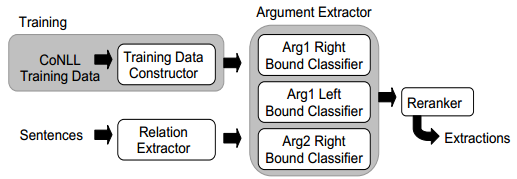
\includegraphics[scale=0.5]{../images/arglearner_architecture.png}
\caption{ArgLearner architecture training and extraction architecture}
\label{fig_arglearner_architecture}
\end{figure}

Furthermore, \textbf{Ollie} (Open Language Learning for Information Extraction) \citep{schmitz2012open} utilizes ReVerb \citep{fader2011identifying} to learn open pattern templates to guide triples extraction from sentence. Additionally, Ollie does a context analysis to extend the tuples with contextual information in order to improve precision \citep{schmitz2012open}. Its training and extraction architecture is describe in Figure \ref{fig_ollie_architecture}.

\begin{figure}
\centering
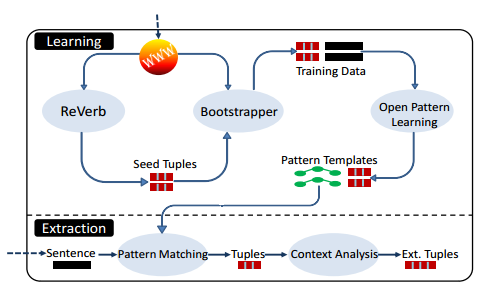
\includegraphics[scale=0.5]{../images/ollie_architecture.png}
\caption{Ollie labeling and extraction architecture}
\label{fig_ollie_architecture}
\end{figure}

One of the most research proposes new open IE system that replaces the usage of large open patterns in Ollie \citep{schmitz2012open} with a set of fewer patterns for canonically structured sentences and a classifier that learns to extract self-contained clauses from a sentence \citep{angeli2015leveraging}. This system is implemented in \textbf{Stanford OpenIE} which is also integrated in the populer open source suites, Stanford Core NLP.

%-----------------------------------------------------------------------------%
\section{\textit{Open Domain Information Extraction}}
%-----------------------------------------------------------------------------%

\lipsum[2-3]

%-----------------------------------------------------------------------------%
\section{\textit{Natural Language Processing}}
%-----------------------------------------------------------------------------%

\lipsum[3]

\subsection{CONLL-U}

\lipsum[4]

\subsection{\textit{Part of Speech Tagging}}

\lipsum[4]

\subsection{\textit{Named-Entity Recognition}}

\lipsum[5]

\subsection{\textit{Dependency Parsing}}

\lipsum[6]

%-----------------------------------------------------------------------------%
\section{\textit{Supervised Learning}}
%-----------------------------------------------------------------------------%

\lipsum[3]

\subsection{\textit{Logistic Regression}}

\lipsum[4]

\subsection{\textit{Support Vector Machine}}

\lipsum[5]

\subsection{\textit{Multi-Layer Perceptron}}

\lipsum[6]

\subsection{\textit{Random Forest}}

\lipsum[7]

\subsection{\textit{Cross Validation}}

\lipsum[8]
